\chapter{Design Methodology}
Define specs; select architecture; perform small-signal and large-signal simulations; run PSS/Pnoise or time-domain jitter; tune \(K_{VCO}\); linearize tuning; validate across PVT; finalize layout.

\section{Meta-Heuristic Optimization (Bonus)}
Apply a simple GA/PSO to choose \(L\), varactor bank size, and bias to minimize a cost combining PN@offsets, power, and tuning coverage. The flow evaluates a fast surrogate (analytical + corner multipliers) and verifies finalists with detailed simulations. Convergence typically occurs in tens of iterations; constraints enforce KVCO and range.

\begin{figure}[H]
  \centering
  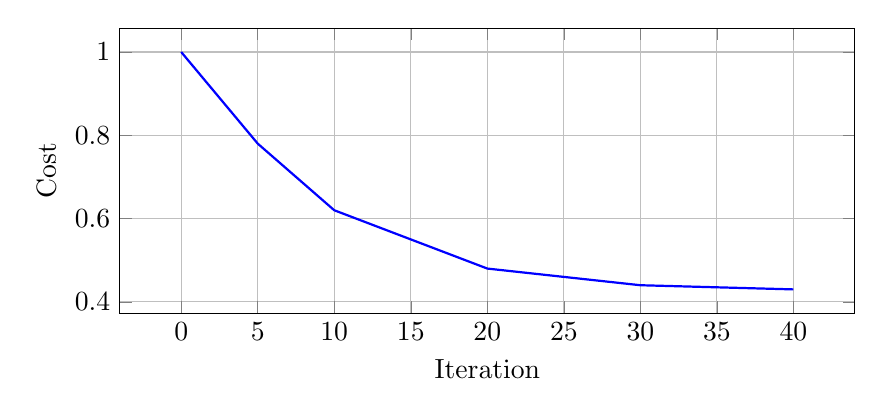
\begin{tikzpicture}
    \begin{axis}[width=0.9\linewidth, height=5.2cm, xlabel={Iteration}, ylabel={Cost}, grid=both]
      \addplot[blue, thick] table[row sep=\\]{x y \\
        0  1.00 \\
        5  0.78 \\
        10 0.62 \\
        20 0.48 \\
        30 0.44 \\
        40 0.43 \\
      };
    \end{axis}
  \end{tikzpicture}
  \caption{Illustrative convergence of a meta-heuristic cost function}
\end{figure}

\section{Step-by-Step Flow}
\begin{enumerate}
  \item Requirements: define PN mask, tuning range, power, spur limits, area.
  \item Architecture choice: ring vs LC; select $L$/$Q$ plan (LC) or stage count (ring).
  \item Initial sizing: set swing, estimate $K_{VCO}$; plan coarse/fine banks and overlap.
  \item Simulation loop: PSS/Pnoise and transient noise; sweep bias and device widths.
  \item Optimization (optional): run GA/PSO on surrogate; verify winners with EM/parasitic.
  \item PVT/Monte Carlo: confirm startup margin, PN spread, spur sensitivity.
  \item Layout and PDN: symmetric routing, guard rings, decoupling networks.
  \item Final validation: measurement hooks, buffer levels, documentation.
\end{enumerate}

\section{Deliverables}
\begin{itemize}
  \item Report with specs, models, results, and comparisons.
  \item Simulation decks and scripts (transient noise, PSS/Pnoise, sweep).
  \item Optional: Python/OCN code for meta-heuristic optimization and data export.
\end{itemize}

\section{Optimization Criteria Matrix}
We combine the main figures of merit (FOMs) in a weighted cost. Typical weights prioritize phase noise while keeping power and range within constraints.
\begin{table}[H]
  \centering
  \begin{tabular}{llll}
    \toprule
    Criterion & Symbol & Target/Constraint & Weight \\
    \midrule
    PN@100 kHz (dBc/Hz) & $\mathcal{L}_{100k}$ & $< -100$ & 0.5 \\
    Power (mW) & $P$ & $< 10$ & 0.2 \\
    Range (\%) & $R$ & $\ge 40$ & 0.2 \\
    $K_{VCO}$ (MHz/V) & $K$ & 1–3 & 0.1 \\
    \bottomrule
  \end{tabular}
  \caption{Example multi-objective weights for meta-heuristic cost}
\end{table}

\section{Optimization Pipeline}
\begin{figure}[H]
  \centering
  \begin{tikzpicture}[node distance=1.6cm, >=Latex]
    \tikzstyle{blk}=[draw, rounded corners, minimum width=3.0cm, minimum height=0.9cm]
    \node[blk] (specs) {Specs & Constraints};
    \node[blk, right=of specs] (sur) {Surrogate Model};
    \node[blk, right=of sur] (ga) {GA/PSO Search};
    \node[blk, right=of ga] (verify) {Detailed Sims (PSS/Pnoise, EM)};
    \node[blk, right=of verify] (pvt) {PVT/MC Sweep};
    \node[blk, right=of pvt] (final) {Finalize & Handoff};
    \draw[->] (specs) -- (sur);
    \draw[->] (sur) -- (ga);
    \draw[->] (ga) -- (verify);
    \draw[->] (verify) -- (pvt);
    \draw[->] (pvt) -- (final);
  \end{tikzpicture}
  \caption{Optimization pipeline from specs to final validated design}
\end{figure}


